\documentclass[proposal]{umthesis}          % for Ph.D. dissertation or proposal
\usepackage{graphicx}% Include figure files
%%\documentclass[thesis]{umthesis}  % for Master's thesis

\usepackage{amsmath}
\usepackage{amsfonts}
\usepackage{float}
\usepackage{epsfig}
%\usepackage[linesnumbered,ruled,vlined]{algorithm2e}

%% If you have enough figures or tables that you run out of space for their
%% numbers in the List of Tables or List of figures, you can use the following
%% command to adjust the space left for numbers.  The default is shown:
%%
%% \setlength{\tablenumberwidth}{2.3em}

\begin{document}
\noindent
A) $\sigma^{2}$ is known and hyperparameter $\mathbf{\alpha}$ is deterministic.

\noindent
First of all, we consider the ideal case that the variance of noise $\sigma^{2}$ is known and the hyperparameter $\mathbf{\boldsymbol{\alpha}} = $ diag $(\alpha_{1}, \alpha_{2}, ... \alpha_{2K})$ which is associated to the source is deterministic. In this case, the source to be estimated is the only unknown variable, we let $\mathbf{x} = [\mathbf{s}]$, where $\mathbf{s}$ denotes the source to be estimated.
With the Bayes' rule and the assumption for $\sigma^{2}$ and $\mathbf{\boldsymbol{\alpha}}$, the likelihood of the measurement $\mathbf{y}$ can be written as 
\begin{align} \label{eqt:likelihood_fisher_1}
P(\mathbf{y,s,\boldsymbol{\alpha}, \sigma^{2}}) = P(\mathbf{y|s,\sigma^{2}})P(\mathbf{s|\boldsymbol{\alpha}})P(\mathbf{\boldsymbol{\alpha}})P(\sigma^{2}),
\end{align}   
where $P(\mathbf{y|s})$ is the likelihood of the measurement and $P(\mathbf{s|\boldsymbol{\alpha}})$ is the prior estimate for the source which appears in the first stage of the hierarchical model, $P(\mathbf{\boldsymbol{\alpha}})$ and $P(\sigma^{2})$ are constant under the assumption and they will be ignored in future analysis.
The natural logarithm of the likelihood (\ref{eqt:likelihood_fisher_1}) is written as 
\begin{align} \label{eqt:loglikelihood_fisher_1}
\log P(\mathbf{y,s,\alpha, \sigma^{2}}) = \log P(\mathbf{y|s})+ \log P(\mathbf{s|\boldsymbol{\alpha}}),
\end{align} 
the expression for $P(\mathbf{y|s})$ is derived in () and $P(\mathbf{s|\boldsymbol{\alpha}})$ is derived in (), (\ref{eqt:loglikelihood_fisher_1}) can be written as 
\begin{equation}
\begin{aligned} \label{eqt:loglikelihood_expansion__fisher_1}
\log P(\mathbf{y,s,\alpha, \sigma^{2}})  = & -M \log \frac{1}{2\pi} - M \log(\sigma)
 - \frac{(\mathbf{y-As})^{T}(\mathbf{y-As})}{2\sigma^{2}} \\
 & - 2K \log \frac{1}{2\pi} - \sum_{i=1}^{2k}\log \sqrt{\alpha_{i}} - \sum_{i=1}^{2k}\frac{s_{i}^{2}}{2\alpha_{i}},
\end{aligned}
\end{equation}
where $M$ is the number of elements and $2K$ is the number of entries in $\mathbf{s}$, the derivative of $\log P(\mathbf{y,s,\alpha})$ with respect to $\mathbf{x}$ is
\begin{equation} \label{eqt:loglikelihood_derivative__fisher_1}
\frac{\partial \log P(\mathbf{y,s,\alpha, \sigma^{2}})}{\partial x} = \frac{\mathbf{A}^{T}(\mathbf{y-As})}{\sigma^{2}} - \sum_{i=1}^{2k}\frac{s_{i}}{\alpha_{i}},
\end{equation}
from (\ref{eqt:loglikelihood_derivative__fisher_1}), we can have the second derivative of the likelihood with respect to x,
\begin{equation} \label{eqt:loglikelihood_second_derivative__fisher_1}
\frac{\partial^{2} \log P(\mathbf{y,s,\alpha, \sigma^{2}})}{\partial x^2} = -\frac{\mathbf{A}^{T}\mathbf{A}}{\sigma^{2}} - \boldsymbol{\alpha}^{-1}.
\end{equation}
According to the definition of the Fisher's matrix (), the Fisher's matrix is obtained by taking the negative expectation, 
\begin{equation} \label{eqt:fishermatrix_fisher_1}
I(\boldsymbol{x}) = \frac{\mathbf{A}^{T}\mathbf{A}}{\sigma^{2}} + \boldsymbol{\alpha}^{-1},
\end{equation}
from (\ref{eqt:fishermatrix_fisher_1}), it can be seen the Fisher's matrix depends on the measurement conditions (i.e., $\mathbf{A}$ and $\sigma^{2}$) and the hyperparameters.
It is known that the lower bound of the estimated variance for the unknown variable is inversely proportional to the Fisher's matrix.
Therefore, it can be concluded that the bound is reduced with the lower $\sigma^{2}$, the more diagnoally dominant matrix $\mathbf{A}^{T}\mathbf{A}$ and $\boldsymbol{\alpha}$ with small values.      

\noindent
B) $\sigma^{2}$ is known and hyperparameter $\mathbf{\alpha}$ is random.

\noindent
Secondly, the sources are drawn from the prior distribution () and the hyperprior distribution is defined in () with the hyperparameter $\lambda$. 
The relationship between the source and the hyperparameter $\lambda$ is obtained by marginalizing out $\mathbf{\alpha}$ where $\mathbf{\alpha}$ is seen as a nuisance parameter, with using the identity (), we can see the distribution of the source is a Laplace distribution with $\lambda$, the distribution is derived in () :
\begin{align} \label{eqt:laplace_prior_fisher_2}
P(\boldsymbol{s} | \lambda ) = \frac{\lambda ^{K}}{2^{2K}} \exp(-\sqrt{\lambda}\sum_{i=1}^{2K}|s_{i}|).
\end{align}  
In this case, there are two unknown variables: $\mathbf{s}$ and $\lambda$, we use $\mathbf{x} = [\mathbf{s}^{T}, \lambda]^{T}$ to denote the two unknown variables. By the definition of the Fisher matrix, it now consists of four blocks,
\begin{equation}
I(\boldsymbol{x}) = \begin{bmatrix}
I(\mathbf{s}) & I(\mathbf{s},\lambda) \\ 
I(\mathbf{s},\lambda)^{T} & I(\lambda)
\end{bmatrix},
\end{equation}
 $I(\mathbf{s}) \in \mathbb{R}^{2k \times 2K} = -\mathop{\mathbb{E}}_{\mathbf{x}} \left \{  \frac{\partial^{2} \log P(\mathbf{y,s,\sigma^{2};\lambda})}{\partial \mathbf{s}^2} \right \}$,
$I(\mathbf{s},\lambda) \in \mathbb{R}^{2k \times 1} = -\mathop{\mathbb{E}}_{\mathbf{x}}\left \{ \frac{\partial^{2} \log P(\mathbf{y,s,\sigma^{2};\lambda})}{\partial \mathbf{s}\partial \lambda}\right \}$ and $I(\lambda)  = -\mathop{\mathbb{E}}_{\mathbf{x}}\left \{ \frac{\partial^{2} \log P(\mathbf{y,s,\sigma^{2};\lambda})}{\partial \lambda^2} \right \}$.
$I(\mathbf{s},\lambda)$ is calculated by the mixed partial derivative, it indicates the correlations between $\mathbf{s}$ and $\lambda$ instead of the variance of these unknown parameters, therefore the expression for $I(\mathbf{s},\lambda)$ will not be derived.
The joint distribution is obtained by combining the likelihood in () and the distribution in (),
\begin{align} \label{eqt:likelihood_fisher_2}
P(\mathbf{y,s,\sigma^{2};\lambda}) \propto  P(\mathbf{y|s,\sigma^{2}})P(\mathbf{s|\lambda})P(\lambda),
\end{align}  
the natural logarithm of the joint distribution is 
\begin{equation}
\log P(\mathbf{y,s,\sigma^{2};\lambda})  = - \frac{(\mathbf{y-As})^{T}(\mathbf{y-As})}{2\sigma^{2}} + (K+1) \log \lambda -\sqrt{\lambda}\sum_{i=1}^{2K}|s_{i}|,
\end{equation}
since $|s_{i}|$ appears in $\log P(\mathbf{y,s,\sigma^{2};\lambda})$, that makes $\log P(\mathbf{y,s,\sigma^{2};\lambda})$ not differentiable with respect to $s_{i}$ when $s_{i} = 0$, here we ignore the case of  $s_{i} = 0$ and consider the other two situations, 
\begin{equation} \label{eqt:first_derivative_s_fisher_2}
\frac{\partial \log P(\mathbf{y,s,\sigma^{2};\lambda})}{\partial s_{i}} = \begin{cases}
 \frac{\mathbf{A_{i}}^{T}(\mathbf{y-A_{i}s})}{\sigma^{2}} -\sqrt{\lambda} & \text{ if } s_{i} > 0 \\ 
 \frac{\mathbf{A_{i}}^{T}(\mathbf{y-A_{i}s})}{\sigma^{2}} + \sqrt{\lambda} & \text{ if } s_{i} < 0 
\end{cases},
\end{equation}
the second term at the right hand side of (\ref{eqt:first_derivative_s_fisher_2}) is independent on $s_{i}$ under the two situations, therefore we can obtain the second derivative of $\log P(\mathbf{y,s,\sigma^{2};\lambda})$ with respect to $\mathbf{s}$ as
\begin{equation} \label{eqt:second_derivative_s_fisher_2}
\frac{\partial^{2} \log P(\mathbf{y,s,\sigma^{2};\lambda})}{\partial \mathbf{s}^2} = -\frac{\mathbf{A}^{T}\mathbf{A}}{\sigma^{2}},
\end{equation}
$I(\mathbf{s})$ is derived by taking the negative expectation of (\ref{eqt:second_derivative_s_fisher_2}), 
\begin{equation}  \label{eqt:fishermatrix_s_fisher_2}
I(\mathbf{s}) = \frac{\mathbf{A}^{T}\mathbf{A}}{\sigma^{2}}.
\end{equation}
It is clear to see compared with bound derived in (\ref{eqt:fishermatrix_fisher_1}), the tighter bound for the variance of estimated $s$ is provided in this case since
\begin{equation}  \label{eqt:fishermatrix_compare_fisher_2}
(\frac{\mathbf{A}^{T}\mathbf{A}}{\sigma^{2}})^{-1} \succeq (\frac{\mathbf{A}^{T}\mathbf{A}}{\sigma^{2}} + \boldsymbol{\alpha}^{-1})^{-1}, 
\end{equation}
another thing we noticed is with $\mathbf{\alpha}$ being marginalized out, the blocks related to $s$ can be computed without knowing the realization of $\mathbf{\alpha}$.
The derivative of $\log P(\mathbf{y,s,\sigma^{2};\lambda})$ with respect to $\lambda$ is
\begin{equation}
\frac{\partial \log P(\mathbf{y,s,\sigma^{2};\lambda})}{\partial \lambda} = \frac{K+1}{\lambda} - \frac{1}{2 \sqrt{\lambda}} \sum_{i=1}^{2K}|s_{i}|,
\end{equation}
then we can have the second derivative is 
\begin{equation} \label{eqt:second_derivative_lambda_fisher_2}
\frac{\partial^{2} \log P(\mathbf{y,s,\sigma^{2};\lambda})}{\partial \lambda^{2}} = -\frac{K+1}{\lambda^{2}} + \frac{1}{4} \lambda^{-\frac{3}{2}} \sum_{i=1}^{2K}|s_{i}|,
\end{equation}
we take the negative expectation of (\ref{eqt:second_derivative_lambda_fisher_2}) to obtain $I(\lambda)$ :
\begin{equation}  \label{eqt:fisher_matrix_block_lambda_fisher_2}
I(\lambda) = - \mathop{\mathbb{E}} \left \{ -\frac{K+1}{\lambda^{2}} + \frac{1}{4} \lambda^{-\frac{3}{2}} \sum_{i=1}^{2K}|s_{i}| \right \} = \frac{K+1}{\lambda^{2}} - \frac{1}{4} \lambda^{-\frac{3}{2}} \mathop{\mathbb{E}} ( \sum_{i=1}^{2K}|s_{i}|), 
\end{equation} 
with the derived distribution for source in (), we can calculate the expected value of $|s_{i}|$
\begin{align}
\mathop{\mathbb{E}} ( |s_{i}|) & = \int_{-\infty }^{\infty } |s_{i}|\cdot p(s_{i},\lambda) ds_{i} = \int_{-\infty }^{\infty }|s_{i}|\frac{\sqrt{\lambda}}{2}\exp(-\sqrt{\lambda}|s_{i}|)ds_{i} \\
& = 2\int_{0 }^{\infty }s_{i}\frac{\sqrt{\lambda}}{2}\exp(-\sqrt{\lambda}s_{i})ds_{i} \\
& = \sqrt{\lambda}\int_{0 }^{\infty }s_{i}\exp(-\sqrt{\lambda}s_{i})ds_{i}\\
& = \frac{1}{\sqrt{\lambda}}, \label{eqt:expectation_of_source}
\end{align} 
plugging (\ref{eqt:expectation_of_source}) into (\ref{eqt:fisher_matrix_block_lambda_fisher_2}), we have 
\begin{equation}  
I(\lambda) = - \mathop{\mathbb{E}} \left \{ -\frac{K+1}{\lambda^{2}} + \frac{1}{4 \lambda^{-\frac{3}{2}}} \sum_{i=1}^{2K}|s_{i}| \right \} = \frac{K+2}{2\lambda^{2}}. 
\end{equation} 
In this case, the lower bound of the variance of sources ($\mathbf{s}$) only depends on measurement matrix $\mathbf{A}$ and noise variance $\sigma^{2}$, the lower bound of the variance for heyperparameter $\lambda$ is proportional on the square of its true value and inversely proportional to the size of the angle grid $K$.

\noindent
c) $\sigma^{2}$ is unknown

\noindent
In this case, the variance of noise $\sigma^{2}$ is unknown, we use $\mathbf{x} = [\mathbf{s}^{T}, \sigma^2]^{T}$ to denote the unknown variables. Now the Fisher matrix is written as  
\begin{equation}
I(\boldsymbol{x}) = \begin{bmatrix}
I(\mathbf{s}) & I(\mathbf{s},\sigma^{2}) \\ 
I(\mathbf{s},\sigma ^{2})^{T} & I(\sigma^{2})
\end{bmatrix},
\end{equation}
for the four blocks of the Fisher matrix, $I(\mathbf{s})$ has been derived in (\ref{eqt:fishermatrix_fisher_1}) when $\mathbf{\alpha}$ is deterministic and (\ref{eqt:fishermatrix_s_fisher_2}) when $\mathbf{\alpha}$ is drawn from the specific distribution, $I(\mathbf{s},\sigma^{2})$ is a zero vector which is not related to the variance of the estimated variable. Therefore, we focus on the block $I(\sigma^{2})$, let $\eta = \sigma^{2}$, 
\begin{equation}
I(\eta) = - \mathop{\mathbb{E}} \left \{ \frac{\partial^{2} \log P(\mathbf{y,s;\eta})}{\partial \eta ^{2}} \right \}
\end{equation}
the second derivative of $\log P(\mathbf{y,s;\eta})$ with respect to $\eta$ is
\begin{equation}
\frac{\partial^{2} \log P(\mathbf{y,s;\eta})}{\partial \eta^{2}} = -\frac{(\mathbf{y-As})^{T}(\mathbf{y-As})}{\eta^{3}},
\end{equation}
since $\mathbf{y-As} = \mathbf{n}$, each entry in $\mathbf{n}$ is assumed to be independent with each other and it is subject to normal distribution with mean zero and variance $\eta$, therefore we can have 
\begin{equation} \label{eqt:y_AS_expectation}
\mathop{\mathbb{E}} \left \{ (\mathbf{y-As})^{T}(\mathbf{y-As}) \right \} = 2M\eta,
\end{equation}
where $M$ is the number of elements. Using (\ref{eqt:y_AS_expectation}), we can compute $I(\eta)$ as :
\begin{equation} \label{eqt:fisher_matrix_block_sigma_fisher_3}
I(\eta) = \frac{2M}{\eta^{2}}.
\end{equation}
In this case, the lower bound of estimated $\sigma^{2}$ is proportional on square of its true variance and inversely proportional to the number of the elements in the receiving system $M$.

\noindent
d) multiple measurements

\noindent
Simulation Results 


The estimated results with various SNR are presented in Figs. \ref{fig:noise_effect_15db_normal} - \ref{fig:noise_effect_30db_normal}.
The normal non-linear array with 12 elements is deployed and 20 experiments are conducted for each case with keeping the incoming source same. In the figures, only the estimated sources at correct angles are plotted for the clarity, but the estimated results at wrong angles are considered when the MSE is calculated with (). 
The value of lower bound ( i.e., inverse of (\ref{eqt:fishermatrix_s_fisher_2})) and MSE in each case are both indicated in the figures. From the figures it is seen that the MSE is always larger than the lower bound and the MSE drops with the increase of SNR.  


\begin{figure}[H]
	\centering
	\includegraphics[width=0.6\columnwidth]{./results/noise_effect_15db_normal}
	\caption{SNR = 15 dB, N = 3, M = 12, L = 10, $\Delta s = 24 \lambda$, $r = 6\lambda$, normal array.}
	\label{fig:noise_effect_15db_normal}
\end{figure}

\begin{figure}[H]
	\centering
	\includegraphics[width=0.6\columnwidth]{./results/noise_effect_20db_normal}
	\caption{SNR = 20 dB, N = 3, M = 12, L = 10, $\Delta s = 24 \lambda$, $r = 6\lambda$, normal array.}
	\label{fig:noise_effect_20db_normal}
\end{figure}

\begin{figure}[H]
	\centering
	\includegraphics[width=0.6\columnwidth]{./results/noise_effect_25db_normal}
	\caption{SNR = 25 dB, N = 3, M = 12, L = 10, $\Delta s = 24 \lambda$, $r = 6\lambda$, normal array.}
	\label{fig:noise_effect_25db_normal}
\end{figure}

\begin{figure}[H]
	\centering
	\includegraphics[width=0.6\columnwidth]{./results/noise_effect_30db_normal}
	\caption{SNR = 30 dB, N = 3, M = 12, L = 10, $\Delta s = 24 \lambda$, $r = 6\lambda$, normal array.}
	\label{fig:noise_effect_30db_normal}
\end{figure}

The cluster non-linear array is also used to test the effect of noise to the variance of estimated sources.

Fig. \ref{fig:effect_sigma_square_to_source} presents performance of the MSE of source under different factors.

\begin{figure}[H]
	\centering
	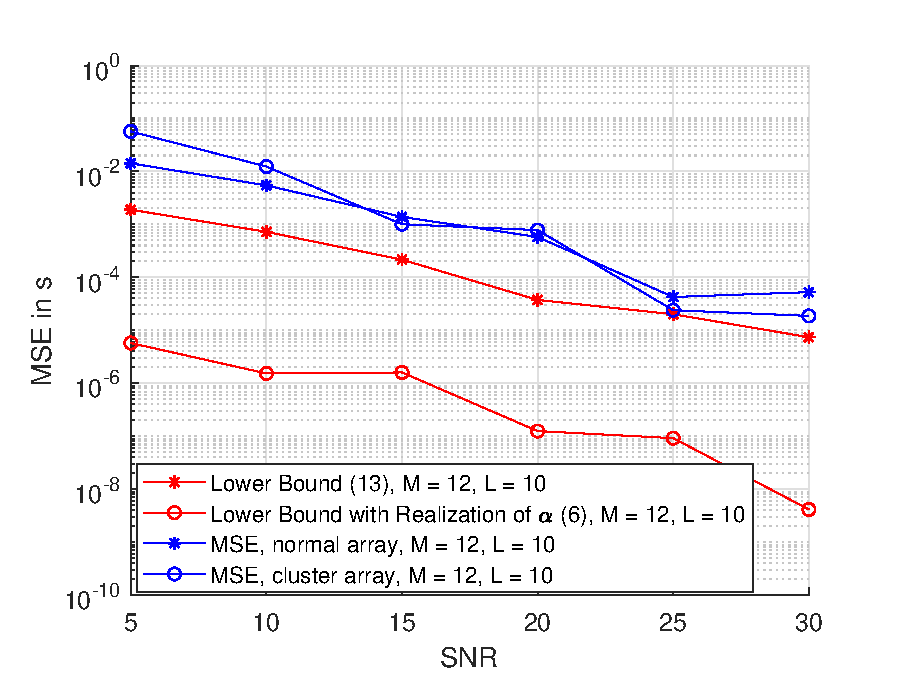
\includegraphics[width=0.6\columnwidth]{./results/change_of_source_with_sigma}
	\caption{N = 3, L = 10}
	\label{fig:effect_sigma_square_to_source}
\end{figure}


Figs. \ref{fig:element_number_effect_6_normal} - \ref{fig:element_number_effect_15_normal} show the estimated results with different number of elements in the array, the normal non-linear array is used and all factors are kept same except the number of elements, in each case we conducted 20 experiments to plot the figures. It can be seen that the variance of the estimated sources decreases with the increase of the number of elements in the array. 
\begin{figure}[H]
	\centering
	\includegraphics[width=0.6\columnwidth]{./results/element_effect_6_normal}
	\caption{SNR = 20 dB, N = 3, M = 6, L = 10, $\Delta s = 24 \lambda$, $r = 6\lambda$, normal array.}
	\label{fig:element_number_effect_6_normal}
\end{figure}

\begin{figure}[H]
	\centering
	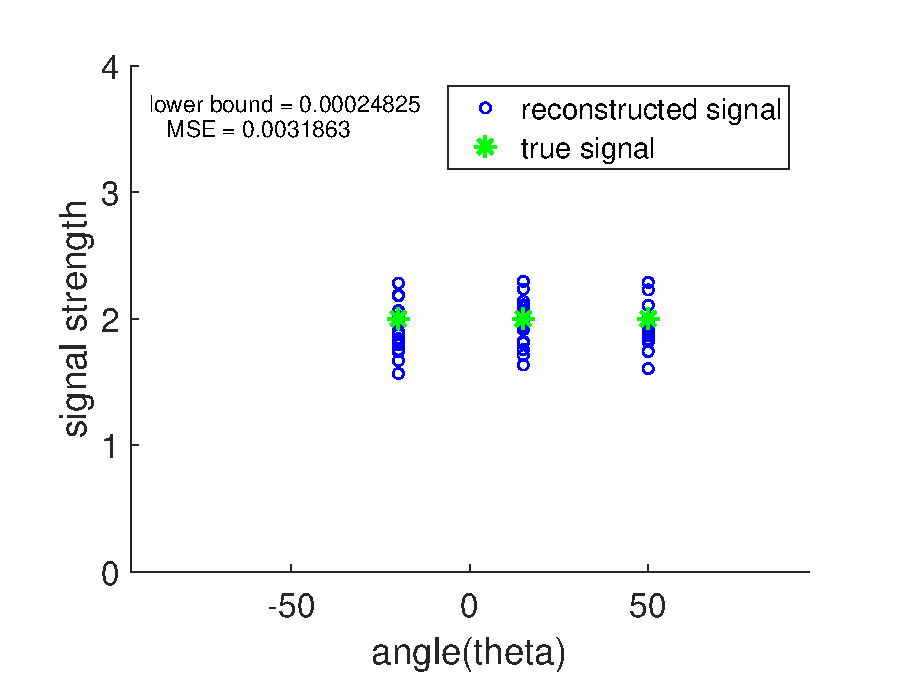
\includegraphics[width=0.6\columnwidth]{./results/element_effect_9_normal}
	\caption{SNR = 20 dB, N = 3, M = 9, L = 10, $\Delta s = 24 \lambda$, $r = 6\lambda$, normal array.}
	\label{fig:element_number_effect_9_normal}
\end{figure}

\begin{figure}[H]
	\centering
	\includegraphics[width=0.6\columnwidth]{./results/element_effect_12_normal}
	\caption{SNR = 20 dB, N = 3, M = 12, L = 10, $\Delta s = 24 \lambda$, $r = 6\lambda$, normal array.}
	\label{fig:element_number_effect_12_normal}
\end{figure}

\begin{figure}[H]
	\centering
	\includegraphics[width=0.6\columnwidth]{./results/element_effect_15_normal}
	\caption{SNR = 20 dB, N = 3, M = 15, L = 10, $\Delta s = 24 \lambda$, $r = 6\lambda$, normal array.}
	\label{fig:element_number_effect_15_normal}
\end{figure}

Figs. \ref{fig:snapshot_effect_5_normal} - \ref{fig:snapshot_effect_50_normal} show the estimated results with different number of measurements, in each measurement, the position of element could change which corresponds to the second case in the subsection of the effect of the number of measurements to the estimated results.
The normal non-linear array is used and all factors are kept same except the number of measurements, in each case we conducted 20 independent experiments to plot the figures.
We can see that the variance of the estimated sources decreases with the increase of the number of measurements which means multiple measurements can provide the more robust results. 

\begin{figure}[H]
	\centering
	\includegraphics[width=0.6\columnwidth]{./results/snapshot_effect_5_normal}
	\caption{SNR = 20 dB, N = 3, M = 12, L = 5, $\Delta s = 24 \lambda$, $r = 6\lambda$, normal array.}
	\label{fig:snapshot_effect_5_normal}
\end{figure}

\begin{figure}[H]
	\centering
	\includegraphics[width=0.6\columnwidth]{./results/snapshot_effect_10_normal}
	\caption{SNR = 20 dB, N = 3, M = 12, L = 10, $\Delta s = 24 \lambda$, $r = 6\lambda$, normal array.}
	\label{fig:snapshot_effect_10_normal}
\end{figure}

\begin{figure}[H]
	\centering
	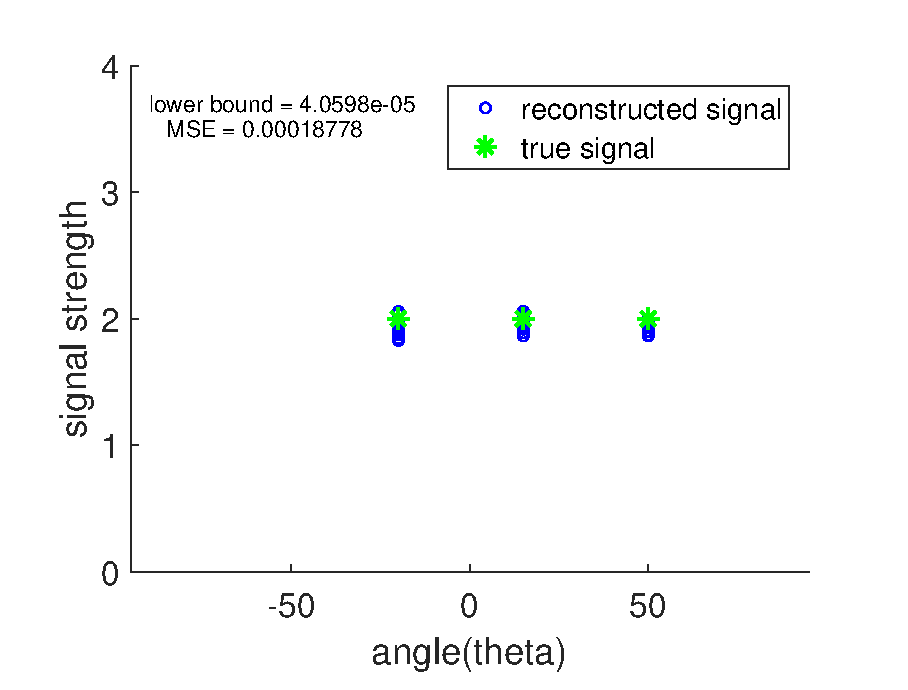
\includegraphics[width=0.6\columnwidth]{./results/snapshot_effect_25_normal}
	\caption{SNR = 20 dB, N = 3, M = 12, L = 25, $\Delta s = 24 \lambda$, $r = 6\lambda$, normal array.}
	\label{fig:snapshot_effect_25_normal}
\end{figure}

\begin{figure}[H]
	\centering
	\includegraphics[width=0.6\columnwidth]{./results/snapshot_effect_50_normal}
	\caption{SNR = 20 dB, N = 3, M = 12, L = 50, $\Delta s = 24 \lambda$, $r = 6\lambda$, normal array.}
	\label{fig:snapshot_effect_50_normal}
\end{figure}

The performance of MSE in $\sigma^{2}$ that estimated with 10 and 50 measurements and normal non-linear array are plotted in Figs. \ref{fig:effect_sigma_square_10_normal} and \ref{fig:effect_sigma_square_50_normal}, respectively. 
The lower bound of the variance of estimated $\sigma^{2}$ under different SNR and receiving antenna array with different number of elements are presented. 
When the number of measurement number is fixed, it can be seen the lower bound and actual MSE both drops with the increase of SNR which matches the expression derived in (\ref{eqt:fisher_matrix_block_sigma_fisher_3}) and they also show more receiving elements is helpful to obtain a better estimation for $\sigma^{2}$.
Compared Fig. \ref{fig:effect_sigma_square_10_normal} with Fig.\ref{fig:effect_sigma_square_50_normal}, we can see the MSE performance of $\sigma^{2}$ is better with more measurements at most cases.    

\begin{figure}[H]
	\centering
	\includegraphics[width=0.6\columnwidth]{./results/change_of_sigma_square_L_10}
	\caption{N = 3, L = 10, $\Delta s = 24 \lambda$, $r = 6\lambda$, normal array.}
	\label{fig:effect_sigma_square_10_normal}
\end{figure}

\begin{figure}[H]
	\centering
	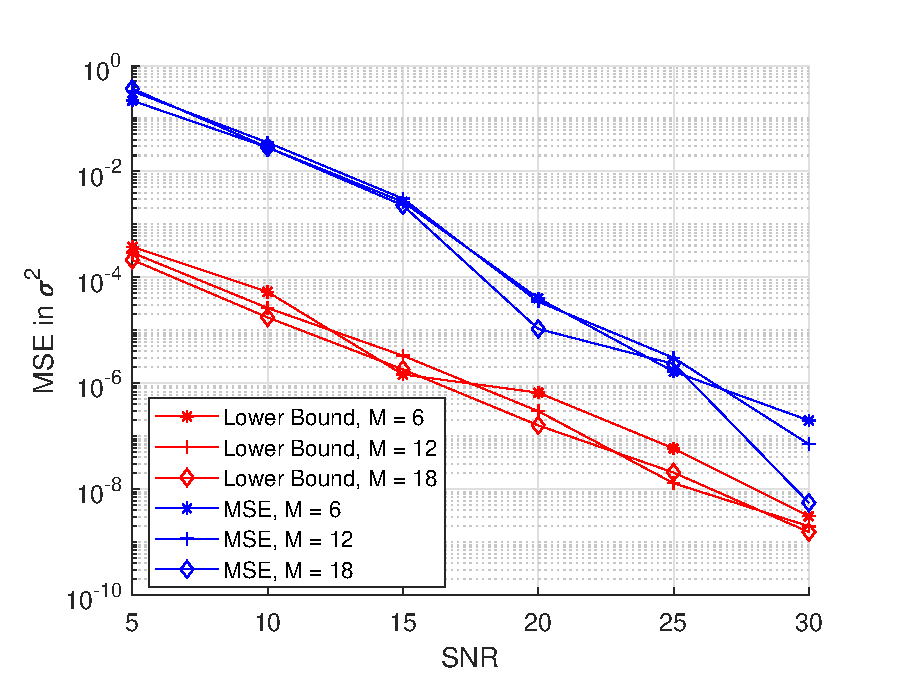
\includegraphics[width=0.6\columnwidth]{./results/change_of_sigma_square_L_50}
	\caption{N = 3, L = 50, $\Delta s = 24 \lambda$, $r = 6\lambda$, normal array.}
	\label{fig:effect_sigma_square_50_normal}
\end{figure}


\bibliographystyle{IEEEtran}
\bibliography{E:/latex_biblio/huabiblio}
\end{document}